\documentclass{report}[12pt]

\usepackage{geometry}[a4paper]
\usepackage{appendix}[toc]
\usepackage{inputenc}[uft8]
\usepackage{fontenc}[T1]
\usepackage{fontspec}
\setmainfont{Libertinus Serif}
\usepackage{bussproofs}
\usepackage{qtree}
\usepackage{amsmath}
\usepackage{amssymb}
\usepackage{amsthm}
\usepackage{tikz-cd}
\usepackage{tipa}
\usepackage{listings}
\usepackage[backend=biber, sorting=ynt, style=alphabetic]{biblatex}
\addbibresource{hispania.bib}
\usepackage{xcolor}
\usepackage{epigraph}
\usepackage{bookmark}
\usepackage{tcolorbox}
\usepackage{colortbl}
\usepackage{mathtools}
\usepackage{stmaryrd}
\usepackage{footnote}
\makesavenoteenv{tabular}
\makesavenoteenv{table}
\usepackage{footmisc}[hang, flushmargin, bottom]
\usepackage{hyperref}
\hypersetup{
  colorlinks=true,
  linkcolor=cyan,
  filecolor=magenta,
  citecolor=violet,
}
\usepackage{graphicx}
\graphicspath{{../pics/}}

\setlength\parindent{0pt}
\setlength\footnotemargin{0pt}

\title{El sueño de mi juventud: \\ Fonología automatizada}
\author{Chen Zhaoyang \\ \texttt{zc23@illinois.edu}}

\begin{document}

\maketitle

\pagebreak

\hspace{0pt}
\vfill

\begin{center}
  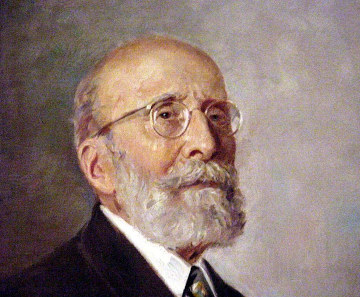
\includegraphics[scale=1.25]{pidal.jpg} \\
  \vspace{0.2cm}
  \Huge{Ramón Menédez Pidal \\ 1869 -- 1968}
\end{center}

\vfill  
\hspace{0pt}

\thispagestyle{empty}

\pagebreak

\begin{abstract}
  
\end{abstract}

\pagebreak

\hspace{0pt}
\vfill

\begin{center}
  \begin{flushleft}
    Lazre clamando secosse mi garganta \\
    canssaron mios oios \\
    sospirando contra mio dios \\
  \end{flushleft}
  \vspace{0.5cm}
  \begin{flushright}
    Salmos LXVIII$\bullet$IV\footnotemark
  \end{flushright}
\end{center}

\footnotetext{\href{https://www.bibliacatolica.com.br/la-biblia-de-jerusalen/salmos/69/}{Estoy exhausto de gritar, arden mis fauces, mis ojos se consumen de esperar a mi Dios.}\begin{flushright} \emph{La Biblia de Jerusalén} Salmos 69:4 \end{flushright} OSp. \emph{Biblia romanceada E8} \cite{osp_tanakh}}

%% \begin{center}
%%   \begin{flushleft}
%%     危冠切浮雲\ 長劍出天外 \\
%%     細故何足慮\ 高度跨一世 \\
%%     非子爲我馭\ 逍遙遊荒裔 \\
%%     顧謝西王母\ 吾將從此逝 \\
%%     豈與蓬戶士\ 彈琴誦言誓 \\
%%   \end{flushleft}
%%   \vspace{0.5cm}
%%   \begin{flushright}
%%     阮籍\ 詠懷第五十八\footnotemark
%%   \end{flushright}
%% \end{center}
%% \footnotetext{\href{https://www.degruyter.com/document/doi/10.1515/9781501503870-004/pdf}{My towering cap touches the drifting clouds, my long sword sticks forth beyond the heavens.  Minor issues are not worth concern, passing on high, I stride across the whole age. Feizi is my carriage driver, free and easy, I roam at the wilderness’s edge. Looking back, I take leave of the Queen Mother, from this point on I will go off. How can I join the gentlemen in a thatched house, plucking a zither and reciting mutual pledges?} Singing My Cares LVIII}

\vfill  
\hspace{0pt}

\pagebreak

\tableofcontents

\pagebreak

\chapter*{Introduction}
\addcontentsline{toc}{chapter}{Introduction}

\epigraph{枯れた技術の水平思考\footnotemark}{横井軍平}
\footnotetext{\href{https://en.wikipedia.org/wiki/Gunpei_Yokoi\#Lateral_Thinking_with_Withered_Technology}{``Lateral Thinking of Withered Technology.''}}

\section*{Seasoned Techniques}

This paper mainly uses \emph{seasoned} techniques in various fields -- meaning that the fundamental works this project builds on have been around for quite some time. \\ The most fundamental technique used here, rule-based phonology, in itself a term coined by its aftecomers, has been around as its \emph{modern} form since at least late \texttt{'}\kern-1pt 60s. \\
The subject of study of this paper, Spanish, whose history belongs to the greater field of Romance historical linguistics; and this is one of the most ripened fruit of European historical linguistics since its birth. Countless literature are still being produced in this field. With all of the excellent works done by our predecessors in this past, a couple of comprehensive monographs on the history of the Spanish language had been produced in English since the later half of the 20\textsuperscript{th} century e.g. \cite{penny_spanish} and \cite{lloyd_spanish}, among many others. This work is not possible without their scholarship. \\
The last piece of the \emph{puzle} [ˈpuθ.le] is \emph{typed programming languages}. Before we touch on anything of that sort, let us talk a little more about (rule-based or not) phonology. At the beginning of the 20\textsuperscript{th} century, phonology, and historical linguisitcs, started to be formalized. After many years of formalization, around and after the publication of \emph{SPE}, the practice of phonology had long acquired a formal language, as we can see from the theoretic elegance and explanatory power of the phonology that was pioneered in \emph{SPE}. Later on in the tradition of \emph{Optimality Theory} \cite{prince_smol_ot} one may say that the formalism within phonology had culminated. \\
So much about phonology again, what does it have to do with typed programming languages? Well, the answer to this question is one of the two themes of this paper, other than giving a concise account of the phonological history of the Spanish language; I want to show that, phonology, which is a formal system, can be simulated by a computer. And this system can be quite naturally implemented in a so-called \emph{high-level programming language}.

\subsection*{Rule-based Phonology}

\subsection*{Romance Historical Linguistics}

\subsection*{Typed Programming Languages}

\section*{Implementation of Phonology}

\chapter*{Notational Conventions}
\addcontentsline{toc}{chapter}{Notational Conventions}

Let us briefly talk about the phonological notations and \emph{pseudocode} conventions used in this paper. The notations used in this paper are not to obfuscate but to illuminate our thoughts; this is the standard that we hold ourselves to.

\section*{Phonological Notations that Diverge from \emph{SPE}}

\subsection*{\textsc{seg} $\vdash$ feat}

For example,
\begin{align*}
  \text{\textipa{T}}\ & \vdash \text{non-sibilant fricative} \\
                     & \vdash \text{dental} \\
                     & \vdash \text{voiceless} 
\end{align*}
The $\vdash$ or $\dashv$ symbol can just be read as ``is'' or ``exhibits the feature \dots''; this is in line with the \emph{SPE} style \cite{spe} notation $\textbf{C}_{\text{[+\ feat]}}$.

\subsection*{[feat$_1$ $\rightarrow$ feat$_2$] \textsc{seg}}

This notation has its roots in the denotation of $\lambda-$calculi and other formal languages, this particular form is adopted from \cite{tpl}. The semantics of this notation is simple: rewrite \textbf{feat}$_1$ to \textbf{feat}$_2$ within \textsc{seg}.
\[ [\text{voiceless} \rightarrow \text{voiced}]\ \text{s} = \text{z} \]

\subsection*{Contexts}

\section*{Pseudocode and Programming Language Misc.}

The pseudocode used in this paper is a \emph{functional} vernacular, which is quite close to the syntax and semantics of real world programming language Haskell \cite{haskell2010} and Standard ML \cite{def_sml}. \\
In any regards, computation is not the focus of this paper, whenever formalism becomes a burden in the clarification of our ideas, we take the liberty to explain them in a natural language.

\subsection*{Functions}

Functions are defined as such.
\begin{align*}
  \text{\textcolor{magenta}{raise}} &\ :\ \texttt{Vowel} \rightarrow \texttt{Vowel} \\
  \text{a} & \Rightarrow \text{e}
\end{align*}
Not so surprisingly, giving \textcolor{magenta}{raise} an [a] would yield an [e].
\[ \text{\textcolor{magenta}{raise}}\ (\text{a} : \texttt{Vowel}) \Rightarrow \text{e} : \texttt{Vowel} \]

\subsection*{Pattern Matching}

Consider this sound change for some hypothetical language that has \{s z n m \textipa{\r*n} \textipa{\r*m}\}.
\begin{align*}
  \text{\textcolor{magenta}{obstruentize}} &\ :\ \texttt{Consonant} \rightarrow \texttt{Consonant} \\
  \textbf{C} \vdash \text{fricative} & \Rightarrow [\text{fricative} \rightarrow \text{stop}]\ \textbf{C} \\
  \textbf{C} \vdash \text{nasal} & \Rightarrow \textbf{match}\ \text{\textcolor{magenta}{voice}}\ \textbf{C}
                                   \begin{cases}
                                     \text{voiced} & \Rightarrow [\text{nasal} \rightarrow \text{stop}]\ \textbf{C} \\
                                     \text{voiceless} & \Rightarrow [\text{nasal} \rightarrow \text{stop};\ \text{unaspirated} \rightarrow \text{aspirated}]\ \textbf{C} \\
                                   \end{cases}
\end{align*}

\begin{align*}
  \text{\textcolor{magenta}{obstruentize}}\ \text{s} & \Rightarrow \text{t} \\
  \text{\textcolor{magenta}{obstruentize}}\ \text{z} & \Rightarrow \text{d} \\
  \text{\textcolor{magenta}{obstruentize}}\ \text{n} & \Rightarrow \text{d} \\
  \text{\textcolor{magenta}{obstruentize}}\ \text{m} & \Rightarrow \text{b} \\
  \text{\textcolor{magenta}{obstruentize}}\ \text{\textipa{\r*n}} & \Rightarrow \text{\textipa{t\super h}} \\
  \text{\textcolor{magenta}{obstruentize}}\ \text{\textipa{\r*m}} & \Rightarrow \text{p\super h} \\
\end{align*}

\begin{align*}
  \lambda &\ :\ \tau \rightarrow \tau \\
  \text{pattern}_0 & \Rightarrow \text{exp}_0 \\
  \vdots & \\
  \text{pattern}_\omega & \Rightarrow \text{exp}_\omega \\
\end{align*}

\begin{align*}
  \textbf{match}\ \text{exp} & \begin{cases}
                                 \text{pattern}_0 & \Rightarrow \text{exp}_0 \\
                                                  & \vdots \\
                                 \text{pattern}_\omega & \Rightarrow \text{exp}_\omega \\
                               \end{cases}\\
\end{align*}

\subsection*{Arity and Currying}

\subsection*{Higher-Order Functions}

\subsection*{Polymorphism}

\part*{Automated Phonology}
\addcontentsline{toc}{part}{Automated Phonology}

\chapter{Statics: Segments, Syllables, and Lexemes}

\epigraph{En el principio existía la Palabra y la Palabra estaba con Dios, y la Palabra era Dios.}{Juan 1:1}

\section{Representation of Segments}

\subsection{Vocalic}

\begin{lstlisting}[basicstyle=\ttfamily, mathescape, escapeinside={(:}{:)}]
  vowel ::= height (:$\times$:) centrality (:$\times$:) duration

  height ::= low | low-mid | mid | high-mid | high

  centrality ::= front | central | back

  duration ::= short | long
\end{lstlisting}

\begin{tabular}{|c|c|c|c|}
  \hline
  & Front & Central & Back \\
  \hline
  High & i & & u \\
  \hline
  High-Mid & \textipa{I} & & \textipa{U} \\
  \hline
  Mid & e & & o \\
  \hline
  Low-Mid & \textipa{E} & & \textipa{O} \\
  \hline
  Low & & a & \\
  \hline
\end{tabular}

\subsection{Consonantal}

\begin{lstlisting}[basicstyle=\ttfamily, mathescape, escapeinside={(:}{:)}]
  consonant ::= manner (:$\times$:) place (:$\times$:) voice

  manner ::= nasal
           | stop
           | fricative
           | non-siblant fricative
           | affricate
           | approximant
           | tap
           | trill
           | lateral

  place ::= bilabial
          | labiodental
          | dental
          | alveolar
          | palatal
          | velar | labiovelar
          | glottal

  place ::= voiced | voiceless
\end{lstlisting}

\section{Representation of Syllables and Lexemes}

\subsection{Syllabic Structure}

\begin{lstlisting}[basicstyle=\ttfamily, mathescape, escapeinside={(:}{:)}]
  syllable ::= onset rhyme

  onset ::= zero-onset
          | monoonset consonant
          | dionset consonant(:$_1$:) consonant(:$_2$:)
          | trionset consonant(:$_1$:) consonant(:$_2$:) consonant(:$_3$:)
          
  rhyme ::= nucleus coda

  nucleus ::= monophthong vowel | diphthong vowel(:$_1$:) vowel(:$_2$:)

  coda ::= zero-coda
         | monocoda consonant
         | dicoda consonant(:$_1$:) consonant(:$_2$:)
\end{lstlisting}

\Tree [.$\sigma$ [.$\Omega$ [.π ] [.$\omega$ ] [.$\mu$ ] ] [.$\rho$ [\qroof{μν. | δφ.}.$\nu$ ] [.K [.$\kappa$ ] [.$\kappa'$ ] ] ] ]

\begin{tabular}{c|c}
  $\omega$ & $\mu$ \\
  \hline
  \begin{tabular}{c}
    p \textipa{B} t d k$^{\text{(w)}}$ g$^{\text{(w)}}$ \\
    f \textipa{T} s x \\
    \textipa{J} \\
    \textipa{\textteshlig} \\
    m n \textipa{\textltailn} \\
    l \textipa{L} \textipa{R} \\
  \end{tabular} & $\varnothing$ \\
  \hline
  \begin{tabular}{c}p b t k g \\ f\end{tabular} & \textipa{R} \\
  \hline
  \begin{tabular}{c}p b t d k g \\ f\end{tabular} & l \\
  \hline
\end{tabular}

\begin{tabular}{c|c}
  $\kappa$ & $\kappa'$ \\
  \hline
  \begin{tabular}{c}
    p t d k \\
    f \textipa{T} s \\
    j \\
    n m \\
    l \textipa{R} \\
  \end{tabular}& $\varnothing$ \\
  \hline
  \begin{tabular}{c}
    p t k \\
    f \\
    n \\
    l \textipa{R} \\
  \end{tabular} & s \\
  \hline
  n & \textipa{T} \\
  \hline
\end{tabular}

\subsection{Syllable Weight and Stress}

Before we can discuss the stress pattern in Latin, it is necessary that we define a function to decide the weight of a syllable in Latin.
\begin{align*}
  \text{\textcolor{magenta}{weight}}\ & :\ \texttt{Syllable} \rightarrow \texttt{Weight} \\
  \sigma\ \vdash \Tree [.\text{$\rho$} [.\text{$\nu$} [.\textbf{V} ] ] [.K [.\text{$\varnothing$} ] ] ] & \Rightarrow \text{light} \\
  \sigma\ \vdash \Tree [.\text{$\rho$} [\qroof{\textbf{V:}\ | δφ.}.\text{$\nu$} ] [.K [.\text{$\varnothing$} ] ] ] & \Rightarrow \text{heavy} \\
  \sigma\ \vdash \Tree [.\text{$\rho$} [.\text{$\nu$} [.\textbf{V} ] ] [.K [.\text{$\kappa$} ] ] ] & \Rightarrow \text{heavy} \\
  \sigma\ \vdash \Tree [.\text{$\rho$} [.\text{$\nu$} [.\textbf{V} ]] [.K [.\text{$\kappa$} ] [.\text{$\kappa'$} ] ] ] & \Rightarrow \text{heavy} \\
\end{align*}
To have a concrete idea, see the following examples.
\begin{align*}
  \text{\textcolor{magenta}{weight}}\ \textsc{s\={o}}_{\dashv\ \textsc{pers\={o}na}} & \Rightarrow \text{heavy} \\
  \text{\textcolor{magenta}{weight}}\ \textsc{men}_{\dashv\ \textsc{fund\={a}mentum}} & \Rightarrow \text{heavy} \\
  \text{\textcolor{magenta}{weight}}\ \textsc{dok}_{\dashv\ \textsc{paradoxus}} & \Rightarrow \text{heavy} \\
  \text{\textcolor{magenta}{weight}}\ \textsc{mi}_{\dashv\ \textsc{similis}} & \Rightarrow \text{light}
\end{align*}
After we are able to decide syllable weight, defining the Latin \textsc{penultimate} stress rule becomes natural.
\begin{align*}
  \text{\textcolor{magenta}{assign stress}}\ & :\ \texttt{List Syllable} \rightarrow \texttt{Lexeme} \\
  [\sigma] & \Rightarrow \begin{aligned}
                                                            & \textbf{let}\ \sigma' = [\text{unstressed} \rightarrow \text{stressed}] \ \sigma \\
                                                            & \textbf{in}\ \text{\textcolor{magenta}{mkLexeme}}\ [\sigma'] \\
                                                          \end{aligned} \\
  [\sigma_1 \dblcolon \sigma_2] & \Rightarrow \begin{aligned}
                                                            & \textbf{let}\ \sigma' = [\text{unstressed} \rightarrow \text{stressed}] \ \sigma_1 \\
                                                            & \textbf{in}\ \text{\textcolor{magenta}{mkLexeme}}\ [\sigma' \dblcolon \sigma_2] \\
                                                          \end{aligned} \\
  [\sigma^{*}]\ \texttt{++}\ [\sigma_1 \dblcolon \sigma_2 \dblcolon \sigma_3] & \Rightarrow \textbf{match}\ \text{\textcolor{magenta}{weight}}\ \sigma_2
                                                      \begin{cases}
                                                        \text{heavy} & \Rightarrow \begin{aligned}
                                                                                     & \textbf{let}\ \sigma' = [\text{unstressed} \rightarrow \text{stressed}]\ \sigma_2 \\
                                                                                     & \textbf{in}\ \text{\textcolor{magenta}{mkLexeme}}\ [\sigma^{*}]\ \texttt{++}\ [\sigma_1 \dblcolon \sigma' \dblcolon \sigma_3] \\
                                                                                   \end{aligned} \\
                                                        \text{light} & \Rightarrow \begin{aligned}
                                                                                     & \textbf{let}\ \sigma' = [\text{unstressed} \rightarrow \text{stressed}]\ \sigma_1 \\
                                                                                     & \textbf{in}\ \text{\textcolor{magenta}{mkLexeme}}\ [\sigma^{*}]\ \texttt{++}\ [\sigma' \dblcolon \sigma_2 \dblcolon \sigma_3] \\
                                                                                   \end{aligned} \\
                                                      \end{cases}
\end{align*}

\subsection{Syllabification}

\chapter{Dynamics: Sound Changes}

%% \epigraph{星翳燈幻露泡夢電雲\footnotemark}{金剛經 \S32}
%% \footnotetext{\href{https://www2.hf.uio.no/polyglotta/index.php?page=record\&vid=1176\&mid=1993243}{A shooting star, a clouding of the sight, a lamp, an illusion, a drop of dew, a bubble, a dream, a lightning’s flash, a thunder cloud.} Diamond Sutra \S32}

\section{Representation of Sound Changes}

\section{Rule Ordering}

\section{Representation of Phonotactics}

\part*{A Phonological History of Spanish}
\addcontentsline{toc}{part}{A Phonological History of Spanish}

\chapter*{Misc. Remarks and Comments}
\addcontentsline{toc}{chapter}{Misc. Remarks and Comments}

\subsection*{Sources for Lat.-Rom.-Es. Gloss.}

\pagebreak

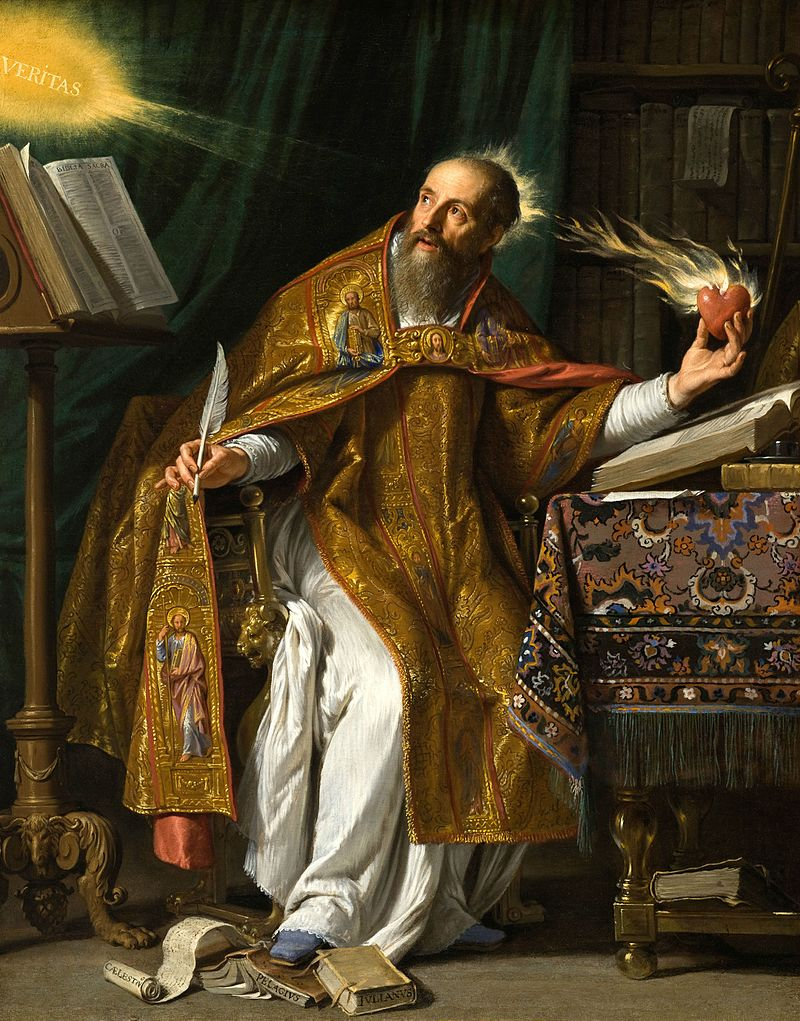
\includegraphics[scale=0.5]{augustine.jpg}

\thispagestyle{empty}

\pagebreak

\chapter{Proto-Romance}

\epigraph{\textsc{finis origine pendent}}{\textsc{marcvs manilivs}}

\section{Phonemic Inventory}

\subsection{Vocalic}

\begin{tcolorbox}[hbox, title=Proto-Romance Monophthongs]
  \begin{tabular}{|c|c|c|c|}
    \hline
    & Front & Central & Back \\
    \hline
    High & i & & u \\
    \hline
    Mid & e & & o \\
    \hline
    Low-Mid & \textipa{E} & & \textipa{O} \\
    \hline
    Low & & a & \\
    \hline
  \end{tabular}
\end{tcolorbox}

\subsection{Consonantal}

\begin{tcolorbox}[title=Proto-Romance Consonants, hbox]
  \begin{tabular}{|c|c|c|c|c|c|c|c|}
    \hline
    & Bilabial & Labiodental & Dental & Alveolar & Palatal & Velar & Labiovelar \\
    \hline
    Nasal & m & & \multicolumn{2}{c|}{n} & \textipa{\textltailn} & & \\
    \hline
    Stop & p \quad b & & t \quad d & & & k \quad g & \textipa{k\super w} \quad \textipa{g\super w} \\
    \hline
    Fricative & \textipa{B} & f & & & \textipa{J} & & \\
    \hline
    \textquotedbl & & & & s \quad z & & & \\
    \hline
    Affricate & & & \textipa{\texttslig} \quad \textipa{\textdzlig} & & \textipa{\textteshlig} \quad \textipa{\textdyoghlig} & & \\
    \hline
    Trill & & & \multicolumn{2}{c|}{r} & & & \\
    \hline
    Lateral & & & \multicolumn{2}{c|}{l} & \textipa{L} & & \\
    \hline
  \end{tabular}
\end{tcolorbox}

\section{Sound Changes}

\subsection{Vocalism}

\begin{tcolorbox}[title=Loss of Quantity, hbox]
  \begin{tabular}{c c}
    \begin{tabular}{|c|c|c|c|c|c|c|}
      \hline
      & \multicolumn{2}{c|}{Front} & \multicolumn{2}{c|}{Cent.} & \multicolumn{2}{c|}{Back} \\
      \hline
      High & \cellcolor{gray} \textsc{\u{i}} & \textsc{\={i}} & & & \cellcolor{gray} \textsc{\u{u}} & \textsc{\={u}} \\
      \hline
      Mid & \cellcolor{gray} \textsc{\u{e}} & \textsc{\={e}} & & & \cellcolor{gray} \textsc{\u{o}} & \textsc{\={o}} \\
      \hline
      Low &  &  & \cellcolor{gray} \textsc{\u{a}} & \textsc{\={a}} & & \\
      \hline
    \end{tabular}
    \quad $\Rightarrow$ & 
                          \begin{tabular}{|c|c|c|c|}
                            \hline
                            & Front & Central & Back \\
                            \hline
                            High & i & & u \\
                            \hline
                            High-Mid & \cellcolor{magenta} \textipa{I} & & \cellcolor{magenta} \textipa{U} \\
                            \hline
                            Mid & e & & o \\
                            \hline
                            Low-Mid & \cellcolor{magenta} \textipa{E} & & \cellcolor{magenta} \textipa{O} \\
                            \hline
                            Low & & a & \\
                            \hline
                          \end{tabular}
  \end{tabular}
\end{tcolorbox}

\begin{tabular}{c c}
  \textsc{latina} & Español \\
  \hline
  \textsc{v\textcolor{red}{\={i}}ta} & v\textcolor{magenta}{i}da \\
  \textsc{vic\textcolor{red}{\={i}}na} & vec\textcolor{magenta}{i}na \\
  \textsc{far\textcolor{red}{\={i}}na} & har\textcolor{magenta}{i}na \\
  \textsc{l\textcolor{red}{\={u}}na} & l\textcolor{magenta}{u}na \\
  \textsc{d\textcolor{red}{\={u}}ra} & d\textcolor{magenta}{u}ra \\
  \textsc{m\textcolor{red}{\={u}}ru} & m\textcolor{magenta}{u}ro \\
  \textsc{h\textcolor{red}{\={o}}ra} & h\textcolor{magenta}{o}ra \\
  \textsc{c\textcolor{red}{\={o}}rte} & c\textcolor{magenta}{o}rte \\
  \textsc{d\textcolor{red}{\={e}}bet} & d\textcolor{magenta}{e}be \\
  \textsc{t\textcolor{red}{\={e}}rnu} & t\textcolor{magenta}{e}rno \\
\end{tabular}

\begin{tcolorbox}[title=Great Merger, hbox]
  \begin{tabular}{c c}
    \begin{tabular}{|c|c|c|c|}
      \hline
      & Front & Central & Back \\
      \hline
      High & i & & u \\
      \hline
      High-Mid & \cellcolor{gray} \textipa{I} & & \cellcolor{gray} \textipa{U} \\
      \hline
      Mid & e & & o \\
      \hline
      Low-Mid & \textipa{E} & & \textipa{O} \\
      \hline
      Low & & a & \\
      \hline
    \end{tabular}
    \quad $\Rightarrow$ &
                          \begin{tabular}{|c|c|c|c|}
                            \hline
                            & Front & Central & Back \\
                            \hline
                            High & i & & u \\
                            \hline
                            Mid & \cellcolor{magenta} e & & \cellcolor{magenta} o \\
                            \hline
                            Low-Mid & \textipa{E} & & \textipa{O} \\
                            \hline
                            Low & & a & \\
                            \hline
                          \end{tabular}
  \end{tabular}
\end{tcolorbox}

\begin{tabular}{c c}
  \textsc{latina} & Español \\
  \hline
  \textsc{g\textcolor{red}{u}la} & g\textcolor{magenta}{o}la \\
  \textsc{c\textcolor{red}{u}rrit} & c\textcolor{magenta}{o}rre \\
  \textsc{m\textcolor{red}{\u{u}}sca} & m\textcolor{magenta}{o}sca \\
  \textsc{b\textcolor{red}{i}b\textcolor{red}{i}t} & b\textcolor{magenta}{e}b\textcolor{magenta}{e} \\
  \textsc{l\textcolor{red}{i}ttera} & l\textcolor{magenta}{e}tra \\
  \textsc{v\textcolor{red}{\u{i}}ce} & v\textcolor{magenta}{e}z \\
\end{tabular}

\begin{tcolorbox}[title=Monophthongization]
  \begin{align*}
    \textsc{oe} & \Rightarrow \text{e} \\
    \textsc{au} & \Rightarrow \text{o} \\
    \textsc{ae} & \Rightarrow \text{\textipa{E}}\ |\ \text{e} \\
  \end{align*}
\end{tcolorbox}

\begin{tabular}{c c}
  \textsc{latina} & Español \\
  \hline
  \textsc{p\textcolor{red}{oe}na} & p\textcolor{magenta}{e}na \\
  \textsc{f\textcolor{red}{oe}du} & f\textcolor{magenta}{e}o \\
  \textsc{\textcolor{red}{au}ru} & \textcolor{magenta}{o}ro \\
  \textsc{thes\textcolor{red}{au}ru} & tes\textcolor{magenta}{o}ro \\
  \textsc{p\textcolor{red}{au}peru} & p\textcolor{magenta}{o}bre \\
  \textsc{p\textcolor{red}{au}cu} & p\textcolor{magenta}{o}co \\
  \textsc{c\textcolor{red}{ae}cu} & c\textcolor{magenta}{ie}go \\
  \textsc{c\textcolor{red}{ae}lu} & c\textcolor{magenta}{ie}lo \\
  \textsc{s\textcolor{red}{ae}ta} & s\textcolor{magenta}{e}da \\
\end{tabular}

There were other diphthongs (\textsc{ei} and \textsc{ov}) that had been merged with long vowels in the Old Latin period \cite[p.~18]{companion_to_latin}:
\begin{quote}
  [F]rom the mid-second century \textsc{bce} the digraphs \textsc{ei} and \textsc{ov}, which earlier spelled inherited diphthongs, spelled the long vowels /iː/ and /uː/ respectively, regardless of their etymological source, e.g. \textsc{[v]eivam} /wiːwam/ ``living'' (\emph{CIL} I\textsuperscript{2}.1837), \textsc{covravervnt} /kuːraːweːrʊnt/ ``oversaw'' (\emph{CIL} I\textsuperscript{2}.1806).
\end{quote}

\begin{tcolorbox}[title=Loss of Hiatus]

\end{tcolorbox}

\begin{tabular}{c c}
  \textsc{lat.} & Es. \\
  \hline
  \textsc{qu\textcolor{red}{i\={e}}tu} & qu\textcolor{magenta}{e}do \\
  \textsc{par\textcolor{red}{i\u{e}}te} & par\textcolor{magenta}{e}d \\
\end{tabular}

\begin{tcolorbox}[title=Syncope]
  
\end{tcolorbox}

\begin{tabular}{c c}
  \textsc{lat.} & Pop. Lat. \\
  \hline
  \textsc{oc\textcolor{red}{u}lu} & \textsc{oclu} \\
  \textsc{auric\textcolor{red}{u}la} & \textsc{oricla} \\
  \textsc{cal\textcolor{red}{i}du} & \textsc{caldu} \\
  \textsc{ang\textcolor{red}{u}lus} & \textsc{anglus} \\
  \textsc{spec\textcolor{red}{u}lum} & \textsc{speclum} \\
  \textsc{vet\textcolor{red}{u}lus} & \textsc{veclus} \\
  \textsc{vir\textcolor{red}{i}dis} & \textsc{virdis} \\
\end{tabular}

\begin{tabular}{c c}
  \textsc{lat.} & Es. \\
  \hline
  \textsc{lep\textcolor{red}{o}re} & liebre \\
  \textsc{i(n)s\textcolor{red}{u}la} & isla \\
  \textsc{vir\textcolor{red}{i}de} & verde \\
\end{tabular}

parab\textcolor{red}{o}la v. parabla \\

\begin{tcolorbox}[title=Apocope]

\end{tcolorbox}

\subsection{Consonantism}

\begin{tcolorbox}[hbox, title=Latin Consonants]
  \begin{tabular}{|c|c|c|c|c|c|c|c|c|}
    \hline
    & Bilabial & Labiodental & Dental & Alveolar & Palatal & Velar & Labiovelar & Glottal \\
    \hline
    Nasal & m & & \multicolumn{2}{c|}{n} & & & & \\
    \hline
    Stop & p \quad b & & t \quad d & & & k \quad g & \textipa{k\super w} \textipa{g\super w} & \\
    \hline
    Fricative & & f & & & & & & \cellcolor{gray} h \\
    \hline
    \textquotedbl & & & & s \quad z & & & & \\
    \hline
    Approximant & & & & & \cellcolor{gray} j & & \cellcolor{gray} w & \\
    \hline
    Trill & & & \multicolumn{2}{c|}{r} & & & & \\
    \hline
    Lateral & & & \multicolumn{2}{c|}{l} & & & & \\
    \hline
  \end{tabular}
\end{tcolorbox}

\begin{tcolorbox}[title=Prothesis in /sC/]

\end{tcolorbox}

This phenomenon is attested in the Visigothic documents \cite[p.~159]{latin_paleography}:
\begin{quote}
  [T]he addition of \emph{i} at the beginning of a word that starts with an \emph{s} followed by another consonant (\emph{iscriptura}), or its suppression by hypercorrection (\emph{sta} for \emph{ista}).
\end{quote}

\begin{tabular}{c c}
  \textsc{lat.} & Es. \\
  \hline
  \textsc{\textcolor{red}{sp}onsa} & \textcolor{magenta}{esp}osa \\
  \textsc{\textcolor{red}{sp}ata} & \textcolor{magenta}{esp}ada \\
  \textsc{\textcolor{red}{st}udiu} & \textcolor{magenta}{est}udio \\
  \textsc{\textcolor{red}{sp}ongia} & \textcolor{magenta}{esp}onja \\
  \textsc{\textcolor{red}{sc}utu} & \textcolor{magenta}{esc}udo \\
\end{tabular}

\begin{tcolorbox}[title=Nasal Liquid Cluster from Syncope]
  
\end{tcolorbox}

\begin{tabular}{c c}
  \textsc{lat.} & Es. \\
  \hline
  \textsc{te\textcolor{red}{ner}u} & tie\textcolor{magenta}{rn}o \\
  \textsc{ge\textcolor{red}{ner}u} & ye\textcolor{magenta}{rn}o \\
  \textsc{tre\textcolor{red}{mul}at} & tie\textcolor{magenta}{mbl}a \\
\end{tabular}

\begin{tcolorbox}[title=Nasal Nasal Cluster from Syncope]
  
\end{tcolorbox}

\begin{tcolorbox}[title=Betacism I]

\end{tcolorbox}

Visigothic spelling exhibits the ``[c]onfusion of \emph{u} and \emph{b} (\emph{haueo} for \emph{habeo}) or vice versa (\emph{pabor} for \emph{pauor})'' \cite[p.~159]{latin_paleography}.

\begin{tcolorbox}[title=Initial Yod Fortition]

\end{tcolorbox}

\begin{tabular}{c c}
  \textsc{lat.} & Es. \\
  \hline
  \textsc{\textcolor{red}{i}ocu} & \textcolor{magenta}{j}uego \quad [x] \\
  \textsc{\textcolor{red}{i}vis} & \textcolor{magenta}{j}ueves \quad [x] \\
  \textsc{\textcolor{red}{i}uvene} & \textcolor{magenta}{j}oven \quad [x] \\
  \textsc{\textcolor{red}{i}udice} & \textcolor{magenta}{j}uez \quad [x] \\
\end{tabular}

\begin{tabular}{c c}
  \textsc{lat.} & Es. \\
  \hline
  \textsc{ma\textcolor{red}{i}us} & ma\textcolor{magenta}{y}o \\
  \textsc{ma\textcolor{red}{i}ore} & ma\textcolor{magenta}{y}or \\
  \textsc{cu\textcolor{red}{i}us} & cu\textcolor{magenta}{y}o \\
\end{tabular}

\begin{tabular}{c c}
  \textsc{lat.} & Es. \\
  \hline
  \textsc{\textcolor{red}{i}acet} & \textcolor{magenta}{y}ace \\
  \textsc{\textcolor{red}{i}am} & \textcolor{magenta}{y}a \\
\end{tabular}

Visigothic document witnesses ``[t]he use of \emph{g} instead of \emph{j} [\dots] (\emph{magor}) or \emph{i} instead of \emph{g} (\emph{inenitor})'', cf. \textsc{maior}, \textsc{genitor} \cite[p.~159]{latin_paleography}.

\begin{tcolorbox}[title=Fortition of /w/ in Germanic Loanwords]
  
\end{tcolorbox}

\begin{tabular}{c c}
  Gm. & Es. \\  
  \hline
  \textcolor{red}{w}isa & \textcolor{magenta}{gu}isa \\
  \textcolor{red}{w}erra & \textcolor{magenta}{gu}erra \\
  \textcolor{red}{w}arten & \textcolor{magenta}{gu}ardar \\
  \textcolor{red}{w}ant & \textcolor{magenta}{gu}ante \\
\end{tabular}

\begin{tcolorbox}[title=Deaspiration]
  
\end{tcolorbox}

We have evidence that initial /h/ already weakens in Latin: ``[i]n metrical texts final vowels are elided before words beginning with /h\textbf{V}/, exactly as before initial /\textbf{V}/.'' \cite[p.~87]{companion_to_latin} \\
An orthographic evidence for this sound change was the fact that the letter <h> sometime was used to indicate hiatus between vowels in inscriptions \cite[p.~18]{companion_to_latin}: \textsc{ahenvm}\footnote{cf. \textsc{a\={e}num}} [aeːnʊm] (\emph{CIL} I\textsuperscript{2}.581), \textsc{ahena}\footnote{cf. \textsc{a\={e}na}} (\emph{CIL} I\textsuperscript{2}.2093).

\begin{tabular}{c c}
  \textsc{lat.} & Es. \\
  \hline
  \textsc{hispalis} & Sevilla
\end{tabular}

\begin{tcolorbox}[title=Nasal Spirant Law]

\end{tcolorbox}

Old Latin inscriptions reflect this change \cite[p.~17]{companion_to_latin}: \textsc{cosol} v. Class. Lat. \textsc{consul}, \textsc{cesor} v. Class. Lat. \textsc{censor} (\emph{CIL} I\textsuperscript{2}.8).

\begin{tcolorbox}[title=Elision of Intervocalic /g/]

\end{tcolorbox}

\begin{tabular}{c c}
  \textsc{lat.} & Es. \\
  \hline
  \textsc{di\textcolor{red}{g}itu} & dedo \\
  \textsc{iam ma\textcolor{red}{g}is} & jamás \\
  \textsc{ma\textcolor{red}{g}istru} & maestro \\
  \textsc{sa\textcolor{red}{g}itta} & saeta \\
  \textsc{pa\textcolor{red}{g}ense} & país \\
  \textsc{c\={o}\textcolor{red}{g}it\={a}re} & cuidar \\
\end{tabular}

\begin{tcolorbox}[title=Elision of Coda /m/]
  
\end{tcolorbox}

The traces of this sound change go back to Old Latin (\emph{CIL} I\textsuperscript{2}.9) \cite[p.~17]{companion_to_latin}: \\
\begin{tabular}{c c}
  Old Lat. & Class. Lat. \\
  \hline
  \textsc{oino} & \textsc{unum} \\
  \textsc{dvonoro} & \textsc{bonorum} \\
  \textsc{optumo} & \textsc{optimum} \\
  \textsc{viro} & \textsc{uirorum} \\
  \textsc{scipione} & \textsc{scipionem} \\
\end{tabular} \\
Also, ``[i]n metrical texts, where the the final syllables of words ending in /\textbf{V}/ $+$ <\textsc{m}> are treated in the same way as those in final /\textbf{V}/, being elided before a following initial /\textbf{V}/.'' \cite[p.~87]{companion_to_latin}

\begin{tcolorbox}[title=Palatalization and Affrication of Dentals]

\end{tcolorbox}

\begin{tabular}{c c}
  \textsc{lat.} & Es. \\
  \hline
  \textsc{\textcolor{red}{di}urnata} & \textcolor{magenta}{j}ornada [x] \\
                & \\
  \textsc{ho\textcolor{red}{di}e} & ho\textcolor{magenta}{y} [j] \\
  \textsc{ra\textcolor{red}{di}u} & ra\textcolor{magenta}{y}o [j] \\
\end{tabular}

\begin{tcolorbox}[title=Palatalization and Affrication of Velars]

\end{tcolorbox}

\begin{tabular}{c c}
  \textsc{lat.} & Es. \\
  \hline
  \textsc{\textcolor{red}{ge}ogeu} & \textcolor{magenta}{J}orge [x] \\
  \textsc{\textcolor{red}{g}eniu} & \textcolor{magenta}{g}enio [x] \\
                & \\
  \textsc{\textcolor{red}{g}emma} & \textcolor{magenta}{y}ema [j] \\
  \textsc{\textcolor{red}{g}eneru} & \textcolor{magenta}{y}erno [j] \\
                & \\
  \textsc{\textcolor{red}{g}ingiva} & encía \\
  \textsc{\textcolor{red}{g}elare} & helar \\
                & \\
  \textsc{le\textcolor{red}{g}e} & le\textcolor{magenta}{y} [j] \\
  \textsc{fu\textcolor{red}{g}it} & hu\textcolor{magenta}{y}e [j] \\
\end{tabular}

\begin{tabular}{c c}
  \textsc{lat.} & Es. \\
  \hline
  \textsc{\textcolor{red}{c}ivitate} & \textcolor{magenta}{c}iudad [\textipa{T}] \\
  \textsc{\textcolor{red}{c}inque} & \textcolor{magenta}{c}inco [\textipa{T}] \\
  \textsc{\textcolor{red}{c}entu} & \textcolor{magenta}{c}iento [\textipa{T}] \\
  \textsc{vi\textcolor{red}{c}ina} &
                                   ve\textcolor{magenta}{c}ina [\textipa{T}]\footnote{cf. Judeo-Spanish \emph{vi\textcolor{magenta}{z}ina} [z]} \\
  \textsc{ia\textcolor{red}{c}ere} &                                   ya\textcolor{magenta}{c}er [\textipa{T}] \\
\end{tabular}

\pagebreak

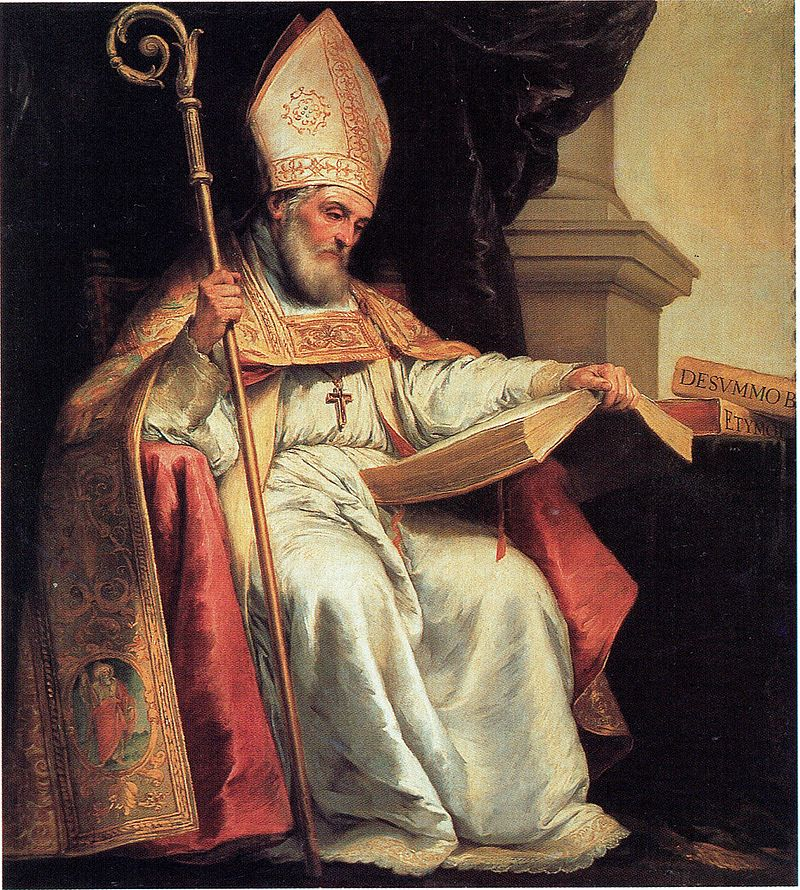
\includegraphics[scale=5.0]{isidorus.jpeg}

\thispagestyle{empty}

\pagebreak

\chapter{Western Romance}

\epigraph{\textsc{venite igitvr descendamvs et confvndamvs ibi lingvam eorvm vt non avdiat vnvsqvisqve vocem proximi svi}}{\textsc{genesis} \textsc{xi}$\bullet$\textsc{vii}}

\section{Phonemic Inventory}

\subsection{Vocalic}

\begin{tcolorbox}[title=Western Romance Monophthongs, hbox]
  \begin{tabular}{|c|c|c|c|}
    \hline
    & Front & Central & Back \\
    \hline
    High & i & & u \\
    \hline
    Mid & e & & o \\
    \hline
    Low & & a & \\
    \hline
  \end{tabular}
\end{tcolorbox}

\subsection{Consonantal}

\begin{tcolorbox}[title=Western Romance Consonants, hbox]
  \begin{tabular}{|c|c|c|c|c|c|c|c|}
    \hline
    & Bilabial & Labiodental & Dental & Alveolar & Palatal & Velar & Labiovelar \\
    \hline
    Nasal & m & & \multicolumn{2}{c|}{n} & \textipa{\textltailn} & & \\
    \hline
    Stop & p \quad b & & t \quad d & & & k \quad g & \textipa{k\super w} \quad \textipa{g\super w} \\
    \hline
    Fricative & \textipa{B} & f & \textipa{D} & & & \textipa{G} & \\
    \hline
    \textquotedbl & & & & s \quad z & & & \\
    \hline
    Affricate & & & \textipa{\texttslig} \quad \textipa{\textdzlig} & & \textipa{\textteshlig} \quad \textipa{\textdyoghlig} & & \\
    \hline
    Trill & & & \multicolumn{2}{c|}{r} & & & \\
    \hline
    Lateral & & & \multicolumn{2}{c|}{l} & \textipa{L} & & \\
    \hline
  \end{tabular}
\end{tcolorbox}

\section{Sound Changes}

\subsection{Vocalism}

\begin{tcolorbox}[title=Diphthongization I]
  
\end{tcolorbox}

\begin{tabular}{c c c}
  \textsc{lat.} & Es. & Fr. \\
  \hline
  \textsc{p\textcolor{red}{e}tra} & p\textcolor{magenta}{ie}dra & p\textcolor{magenta}{ie}rre \\
  \textsc{f\textcolor{red}{e}le} & h\textcolor{magenta}{ie}l & f\textcolor{magenta}{ie}l \\
  \textsc{v\textcolor{red}{e}nit} & v\textcolor{magenta}{ie}ne & v\textcolor{magenta}{ie}nt \\
  \textsc{h\textcolor{red}{e}ri} & a\textcolor{magenta}{ye}r & h\textcolor{magenta}{ie}r \\
\end{tabular}

\subsection{Consonantism}

\begin{tcolorbox}[title=Degemination]
  
\end{tcolorbox}

\begin{tabular}{c c}
  \textsc{lat.} & Es. \\
  \hline
  \textsc{o\textcolor{red}{ss}u} & hue\textcolor{magenta}{s}o \\
  \textsc{su\textcolor{red}{mm}a} & su\textcolor{magenta}{m}a \\
  \textsc{a\textcolor{red}{pp}e\textcolor{red}{ll}at} & a\textcolor{magenta}{p}e\textcolor{magenta}{l}a \\
  \textsc{li\textcolor{red}{tt}era} & le\textcolor{magenta}{t}ra \\
  \textsc{si\textcolor{red}{cc}u} & se\textcolor{magenta}{c}o \\
\end{tabular}

\begin{tcolorbox}[title=Lenition I]
  
\end{tcolorbox}

\begin{tabular}{c c}
  \textsc{lat.} & Es. \\
  \hline
  \textsc{sa\textcolor{red}{p}ore} & sa\textcolor{magenta}{b}or [\textipa{B}] \\
  \textsc{ca\textcolor{red}{p}ut} & ca\textcolor{magenta}{b}o [\textipa{B}] \\
  \textsc{co\textcolor{red}{p}ertu} & cu\textcolor{magenta}{b}ierto [\textipa{B}] \\
                & \\
  \textsc{vi\textcolor{red}{t}a} & vi\textcolor{magenta}{d}a [\textipa{D}] \\
  \textsc{fa\textcolor{red}{t}a} & ha\textcolor{magenta}{d}a [\textipa{D}] \\
  \textsc{ca\textcolor{red}{t}ena} & ca\textcolor{magenta}{d}ena [\textipa{D}] \\
                & \\
  \textsc{ami\textcolor{red}{c}a} & ami\textcolor{magenta}{g}a [\textipa{G}] \\
  \textsc{se\textcolor{red}{c}uru} & se\textcolor{magenta}{g}uro [\textipa{G}] \\
  \textsc{fo\textcolor{red}{c}u} & fue\textcolor{magenta}{g}o [\textipa{G}] \\
\end{tabular}

\begin{tabular}{c c}
  \textsc{lat} & Es. \\
  \hline
  \textsc{ca\textcolor{red}{b}allu} & ca\textcolor{magenta}{b}allo [\textipa{B}] \\
  \textsc{de\textcolor{red}{b}ere} & de\textcolor{magenta}{b}er [\textipa{B}] \\
  \textsc{ha\textcolor{red}{b}ere} & ha\textcolor{magenta}{b}er [\textipa{B}] \\
               & \\
  \textsc{cru\textcolor{red}{d}u} & cru\textcolor{magenta}{d}o [\textipa{D}] \\
  \textsc{pe\textcolor{red}{d}e} & pie \\
               & \\
  \textsc{au\textcolor{red}{g}ustu} & a\textcolor{magenta}{g}osto [\textipa{G}] \\
  \textsc{li\textcolor{red}{g}are} & li\textcolor{magenta}{g}ar [\textipa{G}] \\
  \textsc{pa\textcolor{red}{g}anu} & pa\textcolor{magenta}{g}ano [\textipa{G}] \\
\end{tabular}

\begin{tabular}{c c}  
  \textsc{lat.} & Es. \\
  \hline
  \textsc{le\textcolor{red}{p}re} & lie\textcolor{magenta}{b}re [\textipa{B}] \\
  \textsc{ca\textcolor{red}{p}ra} & ca\textcolor{magenta}{b}ra [\textipa{B}] \\
                & \\
  \textsc{pe\textcolor{red}{t}ra} & pie\textcolor{magenta}{d}ra [\textipa{D}] \\
  \textsc{pa\textcolor{red}{t}re} & pa\textcolor{magenta}{d}re [\textipa{D}] \\
                & \\
  \textsc{hemi-\textcolor{red}{c}rania} & mi\textcolor{magenta}{g}raña [\textipa{G}] \\
\end{tabular}

\begin{tabular}{c c}
  \textsc{lat.} & Es. \\
  \hline
  \textsc{ser\textcolor{red}{p}ente} & ser\textcolor{magenta}{p}iente \\
  \textsc{al\textcolor{red}{p}es} & a\textcolor{magenta}{p}les \\
  \textsc{rum\textcolor{red}{p}ere} & rum\textcolor{magenta}{p}er \\
                & \\
  \textsc{or\textcolor{red}{t}ica} & or\textcolor{magenta}{t}iga \\
  \textsc{men\textcolor{red}{t}a} & men\textcolor{magenta}{t}a \\
                & \\
  \textsc{ar\textcolor{red}{c}u} & ar\textcolor{magenta}{c}o \\
  \textsc{fal\textcolor{red}{c}one} & hal\textcolor{magenta}{c}ón \\
\end{tabular}

The orthography of Visigothic texts shows the signs of lenition \cite[p.~159]{latin_paleography}:
\begin{quote}
  The use of \emph{b} instead of \emph{p} (\emph{abtum}) or \emph{p} for \emph{b} (\emph{puplicum}), \emph{g} for \emph{c} (\emph{eglesia}\footnote{cf. Es. \emph{iglesia}}) or the reverse (\emph{intecritate}), \emph{k} for \emph{c} (\emph{kaput}), \emph{t} for \emph{d} (\emph{aput}) or \emph{d} for \emph{t} (\emph{sustinead}).
\end{quote}

\pagebreak

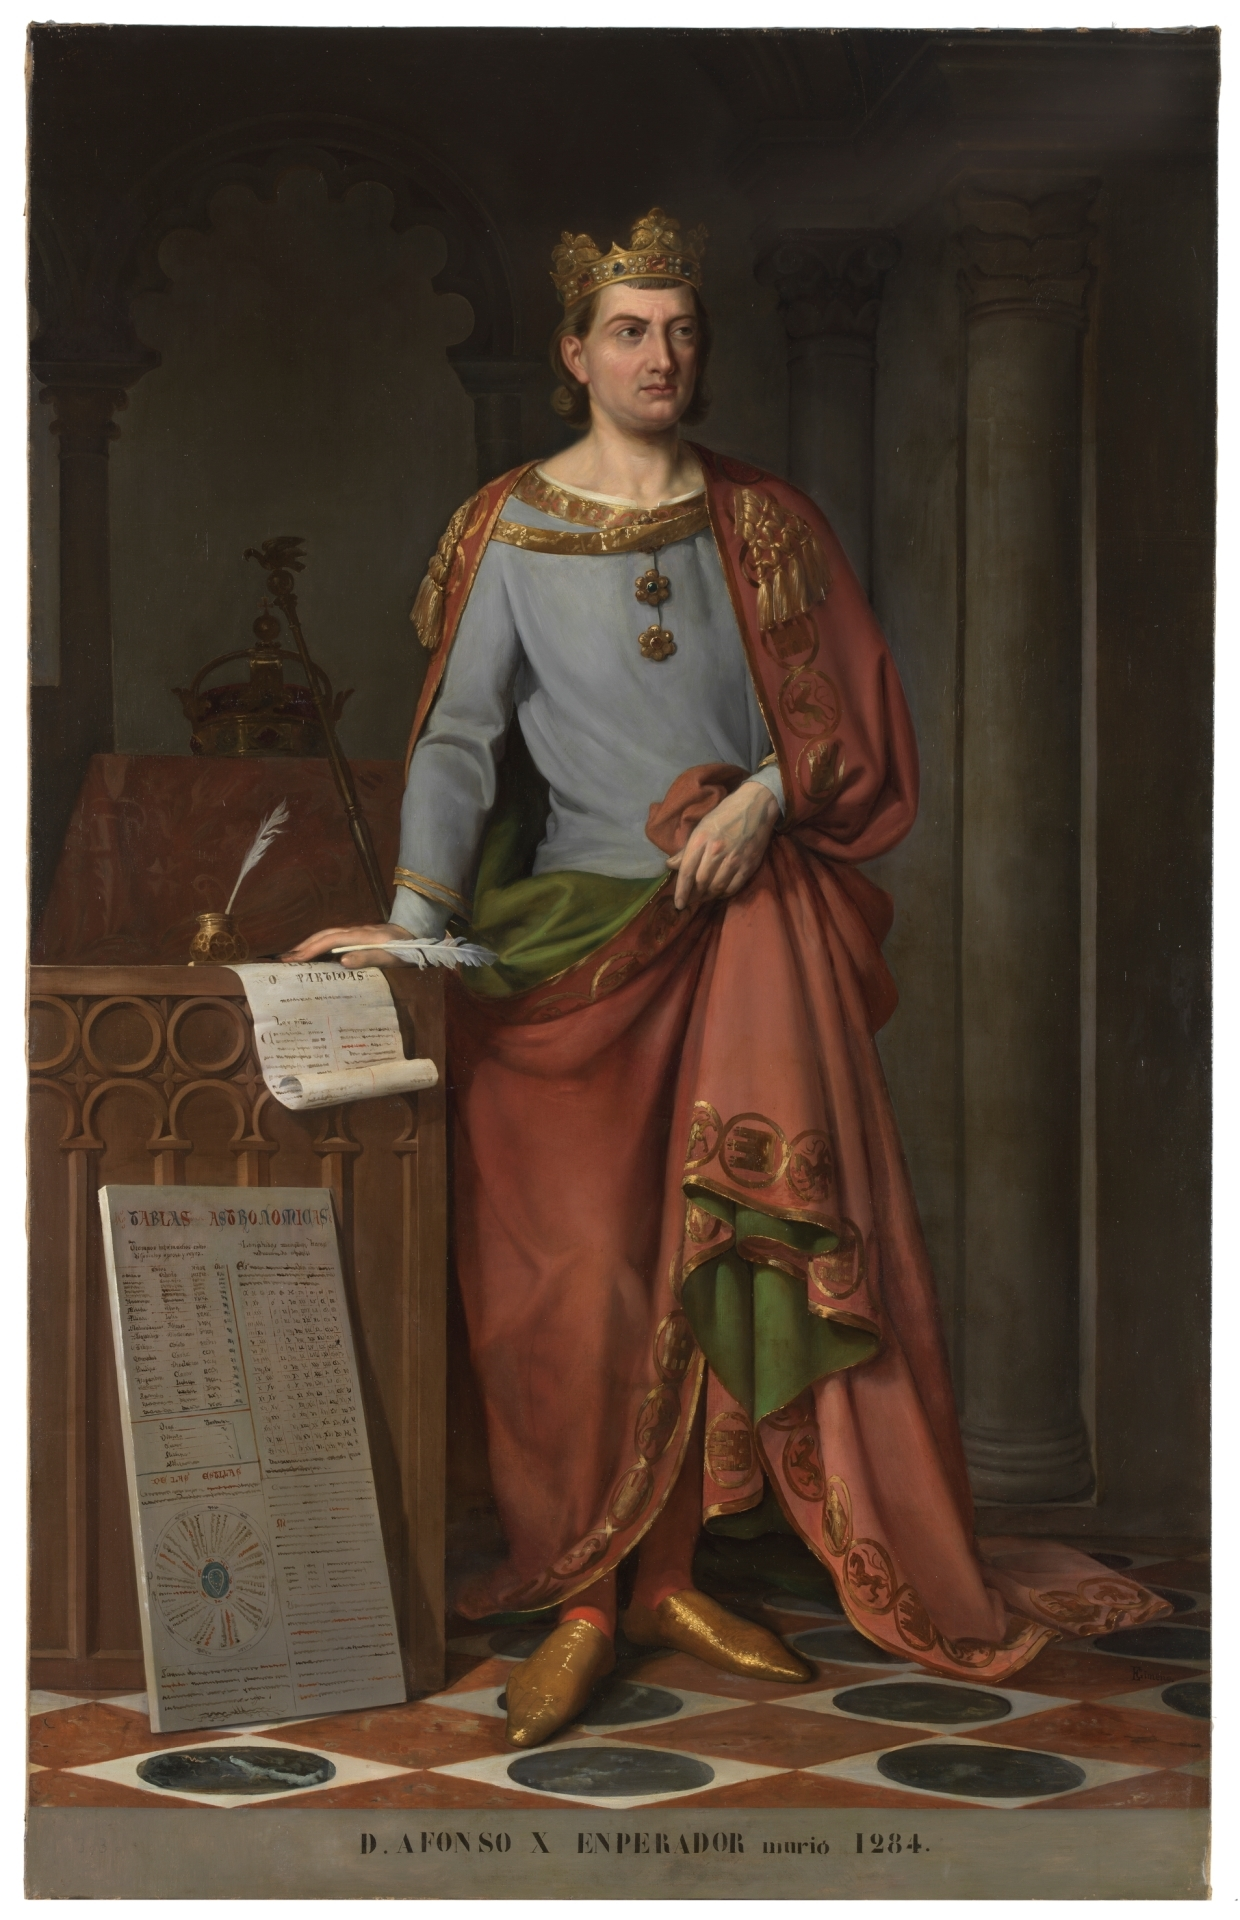
\includegraphics[scale=0.45]{alfonso_x.jpg}

\thispagestyle{empty}

\pagebreak

\chapter{Old Spanish}

% \epigraph{Ya lo vedes, que partirnos emos en vida, yo iré e vós fincaredes remanida.}{Cantar de Mio Cid}

\section{Phonemic Inventory}

\subsection{Vocalic}

\begin{tcolorbox}[title=Old Spanish Monophthongs, hbox]
  \begin{tabular}{|c|c|c|c|}
    \hline
    & Front & Central & Back \\
    \hline
    High & i & & u \\
    \hline
    Mid & e & & o \\
    \hline
    Low & & a & \\
    \hline
  \end{tabular}
\end{tcolorbox}

\subsection{Consonantal}

\begin{tcolorbox}[title=Old Spanish Consonants, hbox]
  \begin{tabular}{|c|c|c|c|c|c|c|c|c|}
    \hline
    & Bilabial & Labiodental & Dental & Alveolar & Palatal & Velar & Labiovelar & Glottal \\
    \hline
    Nasal & m & & \multicolumn{2}{c|}{n} & \textipa{\textltailn} & & & \\
    \hline
    Stop & p \quad b & & t \quad d & & & k \quad g & \textipa{k\super w} \quad \textipa{g\super w} & \\
    \hline
    Fricative & \textipa{F} \quad \textipa{B} & f & \textipa{D} & & \textipa{J} & \textipa{G} & & h \\
    \hline
    \textquotedbl & & & & s \quad z & \textipa{S} \quad \textipa{Z} & & & \\
    \hline
    Affricate & & & \textipa{\texttslig} \quad \textipa{\textdzlig} & & \textipa{\textteshlig} \quad \textipa{\textdyoghlig} & & & \\
    \hline
    Trill & & & \multicolumn{2}{c|}{r} & & & & \\
    \hline
    Tap & & & \multicolumn{2}{c|}{\textipa{R}} & & & & \\
    \hline
    Lateral & & & \multicolumn{2}{c|}{l} & \textipa{L} & & & \\
    \hline
  \end{tabular}
\end{tcolorbox}

\section{Sound Changes}

\subsection{Vocalism}

\begin{tcolorbox}[title=Diphthongization II]
  
\end{tcolorbox}

\begin{tabular}{c c}
  \textsc{lat.} & Es. \\
  \textsc{hib\textcolor{red}{e}rnu} & inv\textcolor{magenta}{ie}rno \\
  \textsc{ap\textcolor{red}{e}rta} & ab\textcolor{magenta}{ie}rta \\
  \textsc{s\textcolor{red}{e}pte} & s\textcolor{magenta}{ie}te \\
  \textsc{c\textcolor{red}{e}rvu} & c\textcolor{magenta}{ie}rvo \\
  \textsc{f\textcolor{red}{e}rru} & h\textcolor{magenta}{ie}rro \\
  \textsc{f\textcolor{red}{o}rte} & f\textcolor{magenta}{ue}rte \\
  \textsc{p\textcolor{red}{o}rta} & p\textcolor{magenta}{ue}rta \\
  \textsc{m\textcolor{red}{o}rdit} & m\textcolor{magenta}{ue}rde \\
  \textsc{m\textcolor{red}{o}rit} & m\textcolor{magenta}{ue}re \\
  \textsc{m\textcolor{red}{o}vet} & m\textcolor{magenta}{ue}ve \\
  \textsc{p\textcolor{red}{o}tet} & p\textcolor{magenta}{ue}de \\
\end{tabular}

\begin{tcolorbox}[title=Metaphony]
  
\end{tcolorbox}

\begin{tabular}{c c}
  \textsc{lat.} & Es. \\
  \hline
  \textsc{m\textcolor{red}{u}ltu} & m\textcolor{magenta}{u}cho \\
  \textsc{ausc\textcolor{red}{u}ltat} & esc\textcolor{magenta}{u}cha \\
  \textsc{l\textcolor{red}{a}cte} & l\textcolor{magenta}{u}cha \\
  \textsc{l\textcolor{red}{a}cte} & l\textcolor{magenta}{e}che \\
  \textsc{f\textcolor{red}{a}ctu} & h\textcolor{magenta}{e}cho \\
  \textsc{b\textcolor{red}{a}siu} & b\textcolor{magenta}{e}so \\
  \textsc{c\textcolor{red}{a}seu} & q\textcolor{magenta}{ue}so \\
  \textsc{r\textcolor{red}{e}ni\={o}ne} & r\textcolor{magenta}{i}ñón \\
  \textsc{g\textcolor{red}{e}nesta} & h\textcolor{magenta}{i}niesta \\
  \textsc{c\textcolor{red}{ae}mentum} & c\textcolor{magenta}{i}miento \\
  \textsc{t\textcolor{red}{e}nebras} & t\textcolor{magenta}{i}nieblas \\
  \textsc{c\textcolor{red}{o}chle\={a}re} & c\textcolor{magenta}{u}chara \\
  \textsc{c\textcolor{red}{o}gn\={a}tu} & c\textcolor{magenta}{u}ñado \\
  \textsc{m\textcolor{red}{u}liere} & m\textcolor{magenta}ujer \\
\end{tabular}

\begin{tcolorbox}[title=Reduction of Final Vowels]

\end{tcolorbox}

\begin{tabular}{c c}
  \textsc{lat.} & Es. \\
  \hline
  \textsc{v\={e}n\={i}} & vine \\  
\end{tabular}

\begin{tabular}{c c}
  OSp. & Es. \\
  \hline
  m\textcolor{red}{ía} & (*m\textcolor{red}{íe} $\rightarrow$) m\textcolor{magenta}{i} \\
  du\textcolor{red}{a}s & du\textcolor{magenta}{e}s \\
  primer\textcolor{red}{o} & primer \\
  tercer\textcolor{red}{o} & tercer \\
  sant\textcolor{red}{o} & san \\
  segund\textcolor{red}{o} & según \\
\end{tabular}

\begin{tabular}{c c}
  \textsc{lat.} & Es. \\
  \hline
  \textsc{pariet\textcolor{red}{e}} & pared \\
  \textsc{merced\textcolor{red}{e}} & merced \\
  \textsc{p\={a}n\textcolor{red}{e}} & pan \\
  \textsc{mar\textcolor{red}{e}} & mar \\
  \textsc{fid\={e}l\textcolor{red}{e}} & fiel \\
  \textsc{p\={a}c\textcolor{red}{e}} & paz \\
  \textsc{calc\textcolor{red}{e}} & coz \\
  \textsc{falc\textcolor{red}{e}} & hoz \\
  \textsc{fasc\textcolor{red}{e}} & haz \\
  \textsc{pisc\textcolor{red}{e}} & pez \\
\end{tabular}

\subsection{Consonantism}

\begin{tcolorbox}[title=Palatalization of Clusters]

\end{tcolorbox}

\begin{tabular}{c c}
  \textsc{lat.} & Es. \\
  \hline
  \textsc{di\textcolor{red}{ct}u} & di\textcolor{magenta}{ch}o [\textipa{\textteshlig}] \\
  \textsc{stri\textcolor{red}{ct}u} & estre\textcolor{magenta}{ch}o [\textipa{\textteshlig}] \\
  \textsc{pe\textcolor{red}{ct}u} & pe\textcolor{magenta}{ch}o [\textipa{\textteshlig}] \\
  \textsc{te\textcolor{red}{ct}u} & te\textcolor{magenta}{ch}o [\textipa{\textteshlig}] \\
  \textsc{no\textcolor{red}{ct}e} & no\textcolor{magenta}{ch}e [\textipa{\textteshlig}] \\
  \textsc{o\textcolor{red}{ct}o} & o\textcolor{magenta}{ch}o [\textipa{\textteshlig}] \\
\end{tabular}

\begin{tcolorbox}[title=Metathesis]

\end{tcolorbox}

\begin{tcolorbox}[title=Debuccalization of /f/]
  
\end{tcolorbox}

\begin{tabular}{c c}
  \textsc{lat.} & Es. \\
  \hline
  \textsc{\textcolor{red}{f}ilu} & \textcolor{magenta}{h}ilo \\
  \textsc{\textcolor{red}{f}erire} & \textcolor{magenta}{h}erir \\
  \textsc{\textcolor{red}{f}erro} & \textcolor{magenta}{h}ierro \\
  \textsc{\textcolor{red}{f}alcone} & \textcolor{magenta}{h}alcón \\
                & \\
  \textsc{\textcolor{red}{f}ocu} & \textcolor{magenta}{f}uego \\
  \textsc{\textcolor{red}{f}ora} & \textcolor{magenta}{f}uera \\
  \textsc{\textcolor{red}{f}onte} & \textcolor{magenta}{f}uente \\
  \textsc{\textcolor{red}{f}ronte} & \textcolor{magenta}{f}rente \\
  \textsc{\textcolor{red}{f}lore} & \textcolor{magenta}{f}lor \\
  \textsc{\textcolor{red}{f}laccu} & \textcolor{magenta}{f}laco \\
\end{tabular}

\pagebreak


\includegraphics[scale=0.75]{marquez.jpg}

\thispagestyle{empty}

\pagebreak

\chapter{Modern Spanish}

\epigraph{Todo está cumplido.}{Juan 19:30}

\section{Phonemic Inventory}

\subsection{Vocalic}

\subsection{Consonantal}

\section{Sound Changes}

\subsection{Vocalism}

\subsection{Consonantism}

\begin{tcolorbox}[title=Lenition II]

\end{tcolorbox}

\begin{tcolorbox}[title=Betacism II]

\end{tcolorbox}

\begin{tcolorbox}[title=Simplication of Clusters]
  
\end{tcolorbox}

\begin{tcolorbox}[title=Deaffrication]

\end{tcolorbox}

\begin{tcolorbox}[title=Devoicing of Fricatives]
  
\end{tcolorbox}

\subsubsection{The Fate of Dental Affricates}

\begin{tcolorbox}[title=Retraction of Palatal Fricative]
  
\end{tcolorbox}

\chapter*{Epilogue: Mein liebster Jugendtraum}
\addcontentsline{toc}{chapter}{Epilogue: \emph{Mein liebester Jugendtraum}}

\epigraph{En adelanto van estos lugares: \\ ya tienen su diosa coronada.}{Leandro Díaz}

\nocite{*}

\chapter*{Bibliography}
\addcontentsline{toc}{chapter}{Biblipgraphy}

\printbibliography[heading=subbibintoc, keyword=phone, title={Phonology}]

\printbibliography[heading=subbibintoc, keyword=romance, title={Romance Linguistics}]

\printbibliography[heading=subbibintoc, keyword=tcs, title={Computation}]

\printbibliography[heading=subbibintoc, keyword=misc, title={Misc.}]

\end{document}
